\documentclass[12pt]{article}
\usepackage{amsmath}
\usepackage{graphicx}
\usepackage{hyperref}
\usepackage[left=2.5cm,top=2.5cm,right=2.5cm,bottom=2.5cm]{geometry} 
\usepackage[portuguese]{babel}
\usepackage{color}

\title{LCOM - Final Report}
\author{Allan Borges de Sousa - 201800149 
\and Juliane de Lima Marubayashi - 201800175}

\begin{document}
\maketitle
\newpage
\section{Instruções de Usuário}
\subsection{Menu}
O jogo começa inicialmente apresentando o menu, o qual expõe ao usuário o nome do jogo e três opções: 
\begin{itemize}
    \item Start
    \item Instructions
    \item Exit
\end{itemize}

\begin{center}
    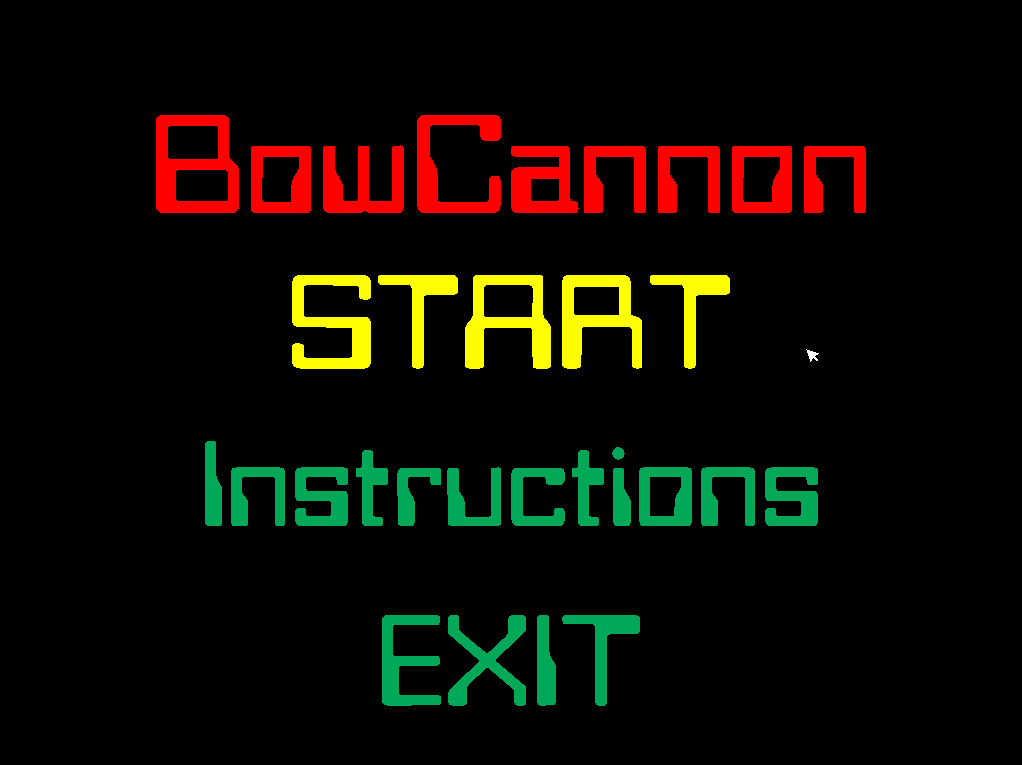
\includegraphics[width = 14cm]{Menu.png}
    \center{\footnotesize{ Fig.1 - Menu}}
\end{center}
\newpage

\subsection{Ask name}
Em seguida ao menu, o jogo pergunta o nome de cada um dos jogadores, para que no final possa
ser exibido o nome do vencedor. É possível apagar o nome e reescrevê-lo. Este módulo foi feito de modo que
o nome seja sempre mostrado no centro do ecrã. 
\begin{center}
    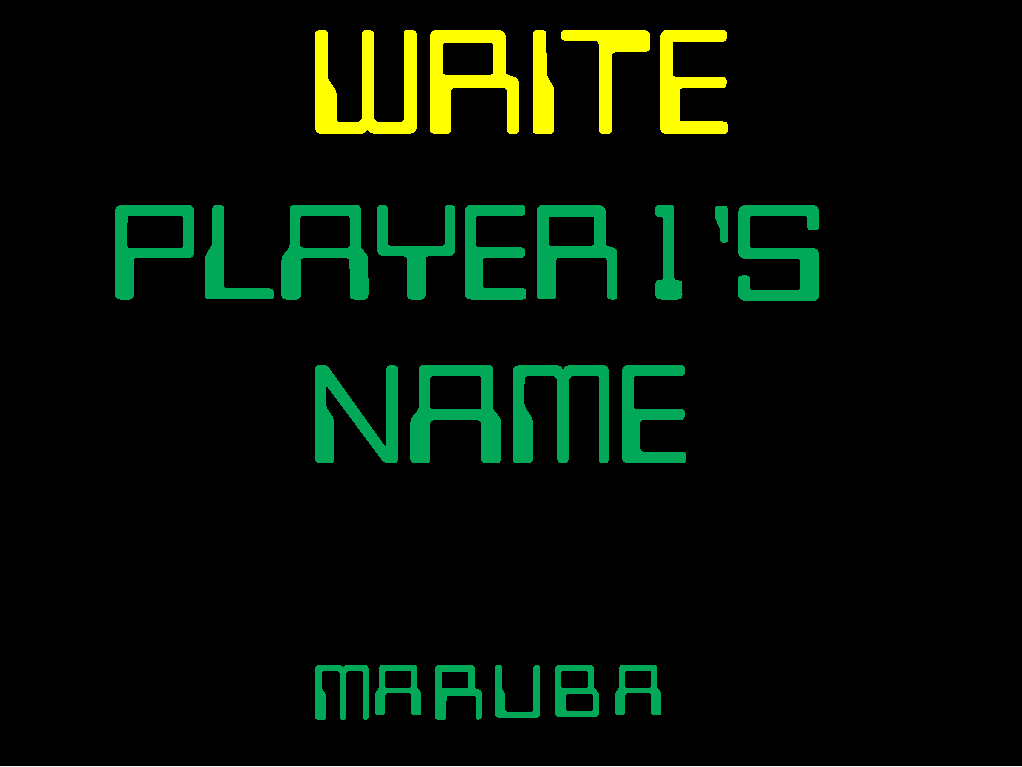
\includegraphics[width = 14cm]{askname.png}
    \center{\footnotesize{ Fig.2 - Jogo pergunta nome}}
\end{center}
\newpage
\subsection{Game - Como funciona}
O jogo deve ser jogado a dois obrigatoriamente. O objetivo é um canhão acertar o outro três vezes e cada vez que um canhão é atingido, ele perde um coração de vida. O ângulo da trajetória do tiro é calculado em relação a posição do mouse.
As regras consistem em:
\begin{itemize}
    \item Os canhões não podem atirar simultânemente;
    \item Uma vez que o canhão da direita atire, por exemplo, é preciso esperar que o canhão da esquerda atire para poder lançar a bola novamente e vice-versa;
    \item Os canhões não podem se aproximar mais do que 300 pixels;
    \item Se um canhão pode ultrapassar os extremos da tela. Esta é uma medida proposital e defensiva. O canhão pode sair da tela, mas enquanto estiver fora não poderá atirar;
    \item Canhões podem mover-se ao mesmo tempo;
\end{itemize}
\begin{center}
	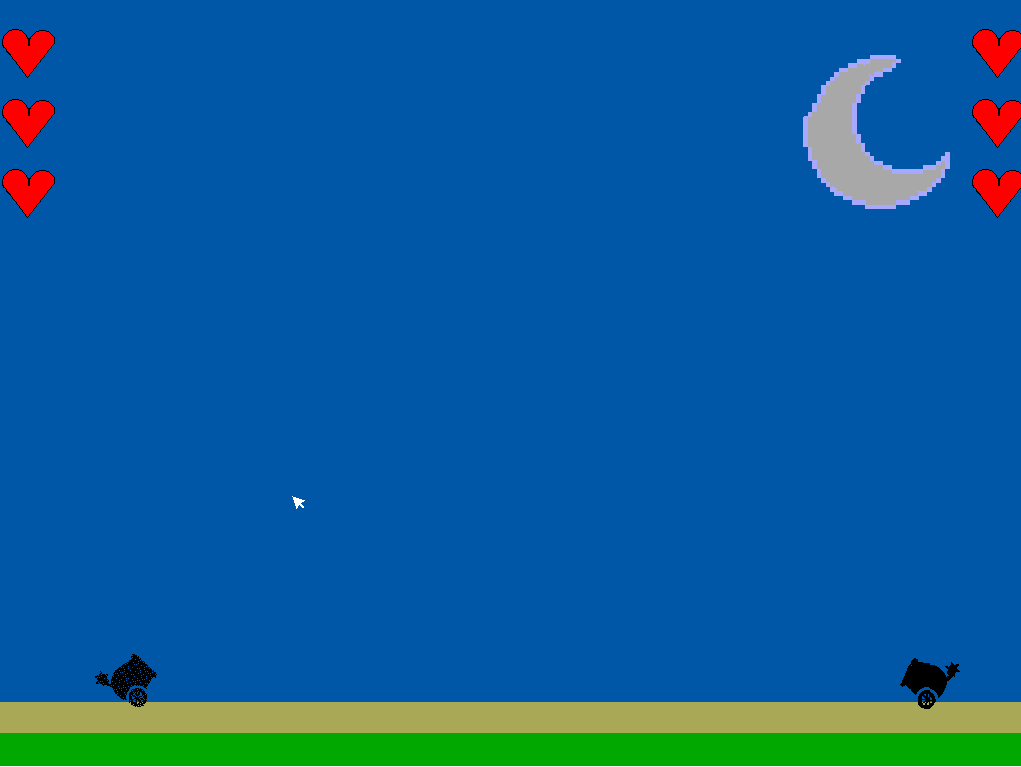
\includegraphics[width = 14cm]{Game_noite.png} 
	\center{\footnotesize{Fig 3 - GamePlay de noite}  
\end{center} 

\begin{center}
    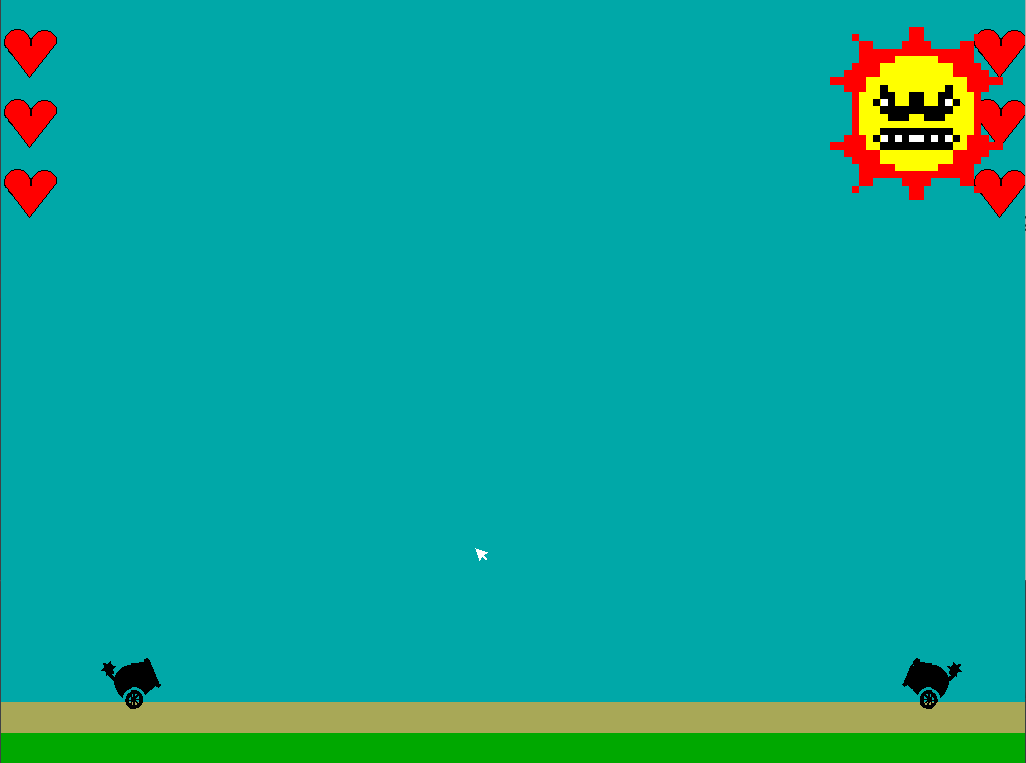
\includegraphics[width = 14cm]{Game.png}
    \center{\footnotesize{ Fig.4 - GamePlay}}
\end{center}
\newpage 
\subsection{Instruções}
Apertando a opção \textbf{Instructions} no menu principal, as instruções do jogo são exibidas.
Resumidamente temos: 
\begin{itemize}
    \item Letras "a" e "d" movem o canhão da esquerda;
    \item Setas da direita e esquerda movem o canhão da direita; 
    \item Posição do rato define o ângulo inicial da parábola da bola do canhão;
    \item Botão esquerdo do rato atira a bola.
\end{itemize} 
\begin{center}
    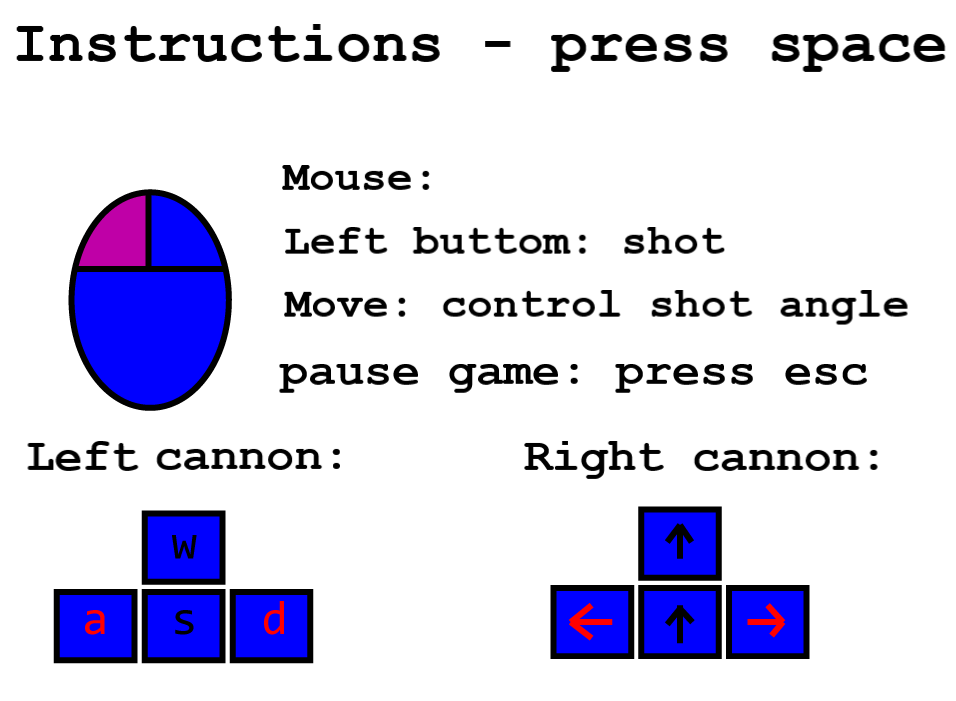
\includegraphics[width = 14cm]{Instructions.png}
    \center{\footnotesize{ Fig.5 - Intruções}}
\end{center}
\newpage
\subsection{Fim de jogo}
Quando um dos canhões perde todos os corações a tela do ecrã muda para e assim que o usuário aperta space, o jogo é reiniciado. 
\newline
\begin{center}
    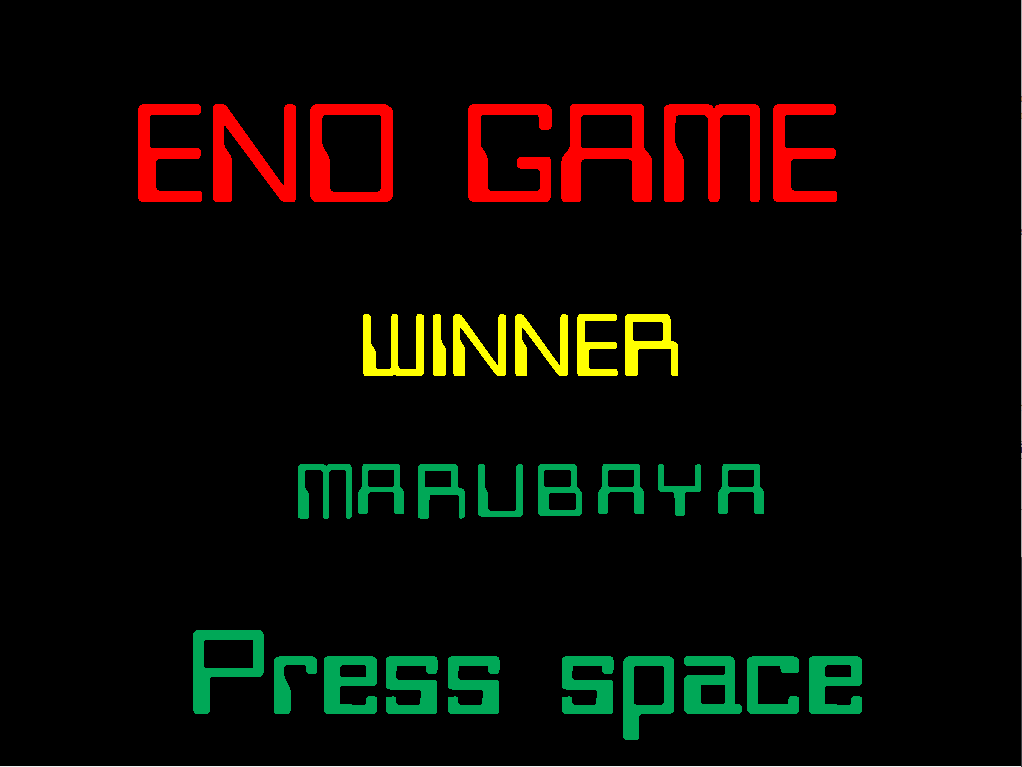
\includegraphics[width = 14cm]{Fim de Jogo.png}
    \center{\footnotesize{Fig.6 - Fim de jogo}}
\end{center}
\newpage
\section{Estado do projeto}
Na tabela a seguir é mostrado resumidamente o uso de cada device no projeto. Detalhes estão descritos em subsections seguintes.
\newline
\begin{center}
    \begin{tabular}{|c|c|c|}
        \hline
        \textbf{Device} & \textbf{Uso} & \textbf{Int.}\\
        \hline
        Timer & Controle do frame rate & S\\
        KBD & Movimento dos canhões & S\\
        Mouse & Movimento do mouse, cáculo de angulo e tiro& S\\
        Video Card & Exibição de imagens& S\\
        RTC & Lê data/hora e faz o update a cada frame& N\\
        \hline
    \end{tabular}
\end{center}

\subsection{Timer}
O timer foi basicamente usado na função \texttt{{\color{blue}int(proj\_main\_loop)(int argc, char *argv[])}}. 
Nesta função, lidamos com os interrupts e a frequência do timer é posta a 64 com a função 
\texttt{{\color{blue}timer\_set\_frequency(0, frequency);}}. \newline
Assim, a cada interrupt do timer a informação do ecrã é atualizada.\newline
Além disso, o timer é responsável por calcular quantos segundos se passaram desde o "inicio" de um tiro, a fim de usar o tempo
na fórmula da trajetória parabólica do tiro, nomeadamete: \newline
$$ s_{x} = vt$$ 
$$s_{y} = s_0+v_0t+\frac{gt^2}{2} \space\space$$ 
$$ g = 9.8$$
O cálculo dos segundos é feito dentro do interrupt do timer. 
\subsection{KBD}
Foi usado para: 
\begin{itemize}
    \item \textbf{Aplicação de controle}
    \item \textbf{Text input}
\end{itemize}
Resumidamente, o kbd tem as seguintes funções: 
\newline
\begin{center}
    \begin{tabular}{|c|c|c|}
        \hline
        Função de cóodigo & Uso & Arquivo\\
        \hline
        \texttt{void handleControls} & Lidar com os movimentos dos canhões & game.c  \\
        \texttt{int(proj\_main\_loop)} & Lidar com mudança de estados do jogo (pause - esc) & proj.c \\
        \texttt{void write\_string} & Escreve a string dada na tela & textInput.c \\ 
        \texttt{void askname1} & Constroi a string digitada pelo usuário & textInput.c \\
        \texttt{char get\_letter} & Retorna a letra digitada pelo usuário & textInput.c e proj.c \\  
        \hline
    \end{tabular}
\end{center}
\newpage
\subsection{Mouse}
Para o mouse foram usados:
\begin{itemize}
    \item \textbf{Posição} (1)
    \item \textbf{Botões} (2)
\end{itemize}
\begin{center}
    \begin{tabular}{|c|c|c|c|}
        \hline
        Função de código& Uso & Arquivo & Tipo\\
        \hline
        \texttt{void animateMouse}& Obter a nova posição do mouse & sprite.c & 1 \\
        \texttt{void get\_angle} & Obter angulo entre a posição do mouse e o canhão & game.c & 1 \\
        \texttt{void check\_start *} & Checar se botão esquerdo foi apertado na área indicada & proj.c & 2 \\
        \texttt{int(proj\_main\_loop)} & Iniciar tiro do canhão & proj.c& 2\\
        \hline
    \end{tabular}
    \small{* void check\_exit e check\_instructions tem basicamente a mesma função}
\end{center}
\subsection{Video Card}
Sobre as características do video card: 
\newline
\begin{center}
    \begin{tabular}{|c|c|c|c|}
        \hline
        Modo & Resolução do ecrã & Modo da cor & Numero de cores\\
        \hline
        0x105 & 1024 x 768 & Indexado & 64\\ 
        \hline
    \end{tabular}
\end{center}
Para a sua implementação foram usados: 
\begin{itemize}
    \item \textbf{Double buffer} (1)
    \item \textbf{Movimento de objetos (detecção de colisões, animação de sprites)} (2)
    \item \textbf{Extra: rotação e inversão de sprites} (3)
    \item \textbf{Exibição de texto e fontes} (4) 
\end{itemize}

Funções utilizadas: 
\begin{center}
    \begin{tabular}{|c|c|c|c|}
        \hline
        Função de código& Uso & Arquivo & Tipo\\
        \hline
        \texttt{void memvideo\_cpy} & Passa informalão do buffer para mem & graphic.c & 1 \\
        \texttt{void malloc\_buffer} & Aloca espaço para o buffer & graphic.c & 1\\  
        \texttt{void clear\_buffer} & Limpa o buffer & graphic.c & 1 \\
        \texttt{int drawPixel} & Desenha pixel no buffer & graphic.c & 1 \\ 
        \texttt{int check\_start} & Vê se a animação do menu inicia deve ser feita & menu.c & 2\\
        \texttt{void cal\_trajetory} & Desenho parabólico do tiro & game.c & 2 \\
        \texttt{void draw\_p1\_hp} & Animação dos corações de vida & game.c & 2 \\ 
        \texttt{int(proj\_main\_loop)} & Animação dos sprites do menu inicial & proj.c & 2 \\
        \texttt{bool checkCollision} & Checa colisão entre bola e canhão & game.c & 2\\ 
        \texttt{int drawSpriteInvertedRotated} & Inverter sprite e rotacionar & sprite.c & 3\\
        \texttt{int drawSpriteRotated} & Rotacionar sprites & sprite.c & 3 \\ 
        \texttt{void drawInvertedSprite} & Inverter sprites & sprite.c & 3 \\
        \texttt{void drawMenu} & Desenhar texto do menu inicial & sprite.c & 4 \\ 
        
        \hline
    \end{tabular}
\end{center}

\subsection{RTC}
Todas as funções do RTC estão implementadas no arquivo rtc.c 
Para sua implementação foram usados: 
\begin{itemize}
    \item \textbf{Leitura da data/hora} (1)
\end{itemize}
\begin{center}
    \begin{tabular}{|c|c|c|c|}
        \hline
        Função de código & Uso & Arquivo & Tipo \\ 
        \hline 
        \texttt{int read\_rtc} & Requisição de leitura da data/ horario & rtc.c & 1 \\
        \texttt{void isDay} & Chamada da função read\_rtc e checa se é dia ou noite & proj.c & 1 \\
        \texttt{int gameDraw} & Desenha sol ou lua de acordo com data/ hora & game.c & 1 \\
        \hline
    \end{tabular}
\end{center}
\subsection{UART}
O uart não foi utilizado no trabalho

\section{Organização e estrutura do código}
{\color{red}Atenção} Módulos não apresentados como timer.c e mouse.c não foram considerados relevantes o 
suficiente para estarem representados em subssecções, uma vez que não sofreram alterações 
significativas em relação aos arquivos produzidos nos labs das aulas práticas. \newline
\subsection{menu.c}
Este submódulo lida com o menu inicial do jogo.\newline
A função principal é a \texttt{void menuDraw} que é responsável por gerir as atividades visuais do menu
que se resumem em:
\begin{itemize}
    \item Desenhar sprites;
    \item Gerir animação dos sprites do menu;
    \item Animar mouse;
    \item Transferir informção do buffer para a memória de vídeo.
\end{itemize}
Podemos dizer que este representa 20\% do trabalho. \newline
Segue a divisão de trabalho para este módulo considerando apenas as funções principais: \newline
\begin{center}
    \begin{tabular}{|r|c|c|}
        \hline
        \textbf{Funções/Componentes} & \textbf{Allan Borges} & \textbf{Juliane Marubayashi} \\ 
        \hline
        \texttt{menuDraw}   & & X \\ 
        \texttt{check functions} & X & \\ 
        \texttt{init\_menuSprites} & X & X \\ 
        \hline
    \end{tabular}
\end{center}


\subsection{game.c}
Este módulo gere o jogo. \newline
A sua função principal é \texttt{int gameDraw} que é responsável por organizar a lógica de jogo e a interface gráfica.
\newline
Sua estrutura de dados principal (definida em sprite.h) é a struct Sprite, que armazena principalmente a velocidade e a posição dos canhões na
interface de jogo. \newline 
\textbf{{\color{red} Atenção}} Esta função não lida totalmente com a jogabilidade. Algumas decisões são tomadas nos interrupts
presentes no módulo proj.c.\newline
Sendo assim, seu percurso programacional é: 
\begin{itemize}
    \item Checar o fim de jogo;
    \item Atualizar posição dos canhões;
    \item Verificar a interface deve ser dia ou noite;
    \item Desenhar no buffer a interface do jogo: canhões, chão, mouse, céu, sol/lua;
    \item Desenhar bola de tiro se necessário;
    \item Mover informação do buffer para a memória de vídeo
\end{itemize}
Podemos dizer que este módulo representa algo em torno de 40\% do trabalho, uma vez que se trata 
da tarefa principal do jogo. 
\begin{center}
    \begin{tabular}{|r|c|c|}
        \hline
        \textbf{Funções/Componentes} & \textbf{Allan Borges} & \textbf{Juliane Marubayashi} \\ 
        \hline
        \texttt{init\_gameSprite} & X & X \\ 
        \texttt{draw\_p1\_hp} & X & \\ 
        \texttt{checkCollision} & X & \\ 
        \texttt{check\_for\_endgame} & X & \\  
        \texttt{gameDraw} & & X \\ 
        \texttt{cannon1\_moviment} & & X \\ 
        \texttt{handleControls} & & X \\ 
        \texttt{draw\_interface} & & X \\ 
        \texttt{cal\_trajectory} & & X \\ 
        \texttt{handle\_shot} & X & X \\ 
        \texttt{get\_angle} & X & \\ 
        \hline
    \end{tabular}
\end{center}
\subsection{textInput.c}
Este módulo é responsável por gerenciar o programa quando pede-se os nomes dos jogadores. \newline
Suas funções principais são \texttt{void askname1()} e \texttt{void askname1()}. \newline
As funções deste módulo foram implementadas por Juliane Marubayashi.  
Consideramos que este módulo representa cerca de 10\% do trabalho total. 
\subsection{proj.c}
Este módulo é responsável pro gerenciar os modos de jogo com base em estados. Além disso, 
nele ocorre a chamada de interrupts e leitura de dados do keyboard e mouse. \newline
Fora as funções mencionadas acima, ainda ocorre: 
\begin{itemize}
    \item Iniciar sprites do menu incial e do jogo;
    \item Definir se o modo do jogo deve ser dia ou noite;
    \item Lidar com interrupts:
    \begin{itemize}
        \item Cálculo dos segundos desde o início de um tiro até seu fim {\color{blue}[TIMER]};
        \item Se state = MENU, desenhar o menu inicial {\color{blue}[TIMER]};
        \item Se state = GAME, desenhar o jogo {\color{blue}[TIMER]} ;
        \item Fazer update do timer a cada frame {\color{blue}[TIMER]}
        \item Se state = PAUSE, o jogo está em pausa e tem a mesma visão do menu principal, mas ao apertar start 
        não é perguntado o nome dos jogadores novamente  {\color{blue}[TIMER]}
        \item Verificar se ESC foi apertado, a fim de voltar ao menu inicial {\color{green}[KBC]};
        \item Colher dados do KBC {\color{green}[KBC]} ;
        \item Se state = NAME1 ou NAME2 é perguntado o nome dos jogadores {\color{green}[KBC]}
        \item Colher dados do rato {\color{red}[MOUSE]};
        \item Verificar opções apertadas no menu inicial {\color{red}[MOUSE]};
        \item Verificar se um tiro deve ser feito {\color{red}[MOUSE]}
    \end{itemize}

\end{itemize}
Este módulo representa algo em torno de \%30 do trabalho. \newline
Divisão do trabalho: \newline 
\begin{center}
    \begin{tabular}{|r|c|c|}
        \hline
        \textbf{Tarefas/Componentes} & \textbf{Allan Borges} & \textbf{Juliane Marubayashi} \\ 
        \hline
        Ler rtc data/ hora & & X \\ 
        Estados & & X \\ 
        Interrupts& X & X \\ 
        \hline
    \end{tabular}
\end{center}

\subsection{xpm.h}
Este arquivo possui todos os xpm utilizados no trabalho. \newline
Para os xpms para os quais foram adquiridos na internet, as fontes estão
no fim deste relatória ne sessão de fontes. 

Este arquivo representa cerca de 10\% considerando principalmente o tempo que levamos para
criar os xpms. \newline
Os xpm's foram criados em conjuntos. Cada componente da dupla compôs cerca de metade dos xpm's
presentes no arquivo. 
\section{Detalhes de implementação}

Para o projeto, usamos e adquirimos mais conhecimento relativo aos seguintes tópicos: 
\begin{itemize}
    \item State machine: usado para mudança de estados dos jogo entre gamemode, menu e gameover. 
    \item Frame generation 
    \item Rotação de sprites utilizando matriz de rotação 
    \item Inversão de sprites 
    \item Aprendemos a criar sprites a partir de pixel art utilizando outros softwares
    \item Colisão de sprites
    \item Animação de sprites 
    \item Orientação de objetos, uma vez que a informação dos canhões era encapsulada em structs. 
    \item Escrita em latex
\end{itemize}
\subsection{Detalhes sobre o rtc} 
O jogo se baseia nas estações no ano e na hora para definir se a interface gráfica deve ser noite ou dia, uma vez que há divergencia
na hora em que o sol se põe e nasce entre as estações do ano. Assim, no arquivo proj.c lidamos com tais divergencias, para que a 
interface dia-noite seja o mais coerente possível. 
\newpage 
\section{Conclusão} 
Com o fim do projeto, tivemos grande aproveitamento da cadeira e sentimos que com este jogo, fomos capazes de testar nossos conhecimentos adquiridos com
os trabalhos laboratoriais. \newline 
\subsection{Sugestões de melhoria}
Acreditamos que as aulas teóricas poderiam ter mais exemplos de demostração de código, uma vez que ajudaria no engajamento da matéria. \newline
Sugerimos também abordar o UART em aulas laboratorias. \newline 

\section{Fontes}
\subsection{Imagens}
\href{https://www.freepik.com/free-icon/circus-cannon_770308.htm}{Canhão}: https://www.pixilart.com/art/angry-sun-mario-3-294e69de4b0e53d\newline
\href{https://www.pixilart.com/art/angry-sun-mario-3-294e69de4b0e53d}{Sol}: https://www.pixilart.com/art/angry-sun-mario-3-294e69de4b0e53d 
\subsection{Ferramentas Online}
\href{https://www.pixilart.com/draw}{PIXELART} : https://www.pixilart.com/draw \newline


\end{document}
